\documentclass[letterpaper,twocolumn,10pt]{article}
\usepackage{usenix-2020-09}

% to be able to draw some self-contained figs
\usepackage{tikz}
\usepackage{amsmath}

% inlined bib file
\usepackage{filecontents}
\newcommand{\citationneeded}{\textsuperscript{\color{blue} [citation needed]}}


%-------------------------------------------------------------------------------
\begin{document}
%-------------------------------------------------------------------------------

%don't want date printed
\date{}

% make title bold and 14 pt font (Latex default is non-bold, 16 pt)
\title{\Large \bf Solving for Fun: Balancing Incremental Game Pacing with Constraint Programming and Evolutionary Algorithms}

%for single author (just remove % characters)
\author{
{\rm Dustin Randall}\\
Eastern Washington University
} % end author

\maketitle

\section{Problem}
\subsection*{Interest} 
Incremental Video Games

\subsection*{Topic} 
Tools for balancing Game Economies within incremental video games.

\subsection*{Question} 
Can we establish a relationship between content, total play time, and the expected time between purchases?

\subsection*{Problem} 
I think the problem is going to be building a tool that empowers game designers
to balance the game economy in single-player incremental games.

\subsection*{What kind of project is this?} 
I believe this project falls under the 'build a system' category.
I would want to build a system that takes in game parameters and provides a balance score.
The other side of this system would be a tool that generates valid game economies based on pacing constraints.
These tools would work together to help game designers create and refine game economies in incremental games.

\subsection*{Obstacles} 
This is generally not a well researched area, and has limited existing literature.
\subsection*{What data is needed?} 
Need to be able to quantify aspects of incremental video game economies.
Additionally, data on constraint solving and optimization search techniques would be useful for validation.


\section{Find a Journal}
I found articles from IEEE Transactions on Games which has an h5-index of 33 according to Google Scholar,
and a D-index of 18 according to research.com. 
While these numbers don't immediately suggest that the journal is top-tier, 
I believe that some credibility can be inferred from the connection with the IEEE organization.
Because games are relatively underrepresented in traditional academic research,
we can consider a journal like this one to be very niche.
I found Using Evolutionary Algorithms to Balance Incremental Game Economies~\cite{rogers_using_2023}
as a reference in GEEvo.~\cite{rupp_geevo_2024}

\section{Conferences}
I found papers from two different conferences related to game design and incremental games.
Playing to Wait~\cite{alharthi_playing_2018} comes from Conference on Human Factors in Computing Systems (CHI).
CHI is relatively unknown with an h5-index of 16 according to Google Scholar, and doesn't appear on research.com.
I found Playing to Wait as a reference in~\cite{rogers_using_2023}

GEEvo~\cite{rupp_geevo_2024} comes from the IEEE Congress on Evolutionary Computation (CEC).
CEC appears to be much better known with an h5-index of 94 on Google Scholar, though it also doesn't appear on research.com.
I found GEEvo in a search from Consensus.app, looking for Incremental Games Economy Balancing

\section{Background}
Most games have some form of economy.~\cite{rogers_using_2023}
These economies come in a variety of forms such as experience points in RPGs, 
units in strategy games, ability gauges in fighting games, ammunition in FPS games, and gold in many other games.
Balancing these economies is a critical aspect in game design and is directly tied to the game's difficulty.~\cite{rogers_using_2023}
One genre of games where the economy is particularly central to the gameplay experience is incremental games.

Incremental and idle games have become popular in recent years in part because they fill 'microboredom' events in our lives.~\cite{alharthi_playing_2018}
While these terms are often used interchangeably, it is helpful to distinguish between them for the purpose of this paper.
Alharthi et al. define idle games as games which are largely or entirely automated, and incremental games as games focused on accumulating resources to generate more resources.~\cite{alharthi_playing_2018}
Another way of phrasing this is "the defining feature of incremental games are numbers that increase at an incrementally increasing rate."~\cite{schmalzer_ontology_2020}

In the context of incremental games, resources are typically represented as numbers that increase over time.
Because incremental games often strip away most other elements of gameplay,~\cite{schmalzer_ontology_2020} "Balancing resource production rates and costs is a critical element of idle games."~\cite{alharthi_playing_2018}
Many incremental games rely on the fact that polynomial functions grow slower than exponential functions, and model producers as polynomial functions, and costs as exponential functions.~\cite{pecorella_math_2016}
For example a single resource with polynomial income and exponential cost may look like Figure~\ref{fig:income_vs_cost},
If we convert the Y axis to log scale, we can see the cost to income ratio continues to grow over time as shown in Figure.~\ref{fig:log_scale}
Much of the fun in incremental games comes from complex interactions between multiple resources with independent income multipliers, such as the figure from Pecorella et al.~\cite{pecorella_math_2016}~\ref{fig:interesting_progression}

One form of indirect currency that all games have is the player's time.~\cite{rupp_geevo_2024}
This currency is why pacing is an important design consideration.
Incremental and idle games take advantage of this by designing gameplay so that the player is never not playing.~\cite{alharthi_playing_2018}
Games like RPGs often reach a 'grinding' stage where the player must repeatedly perform low-reward actions to progress,
but incremental games effectively assign the grinding task to the computer.~\cite{schmalzer_ontology_2020}
A traditional incremental game will have a fixed amount of content, but this content is extended by using a prestige system,
which encourages players to reset their progress and restart from the beginning in exchange for additional resource multipliers.~\cite{alharthi_playing_2018}
"Prestige allows the player to get farther through the cost curve before falling behind."~\cite{pecorella_math_2016}

Beyond the traditional 'single resource' incremental game, another approach taken is the 'derivative' incremental game.~\cite{alharthi_playing_2018}
A derivative incremental game is one where resources can be used to produce additional resource generators.
If Gen1 produces the main resource, Gen2 might produce additional Gen1 instances, and Gen3 would produce Gen2.
This series of resource generators ends up producing an income approaching $e^x$ over time.~\cite{pecorella_math_2016}
This approach still relies on a finite amount of purchases allowing the cost function to eventually outpace the income, preventing infinite growth.

This balance between resource acquisition and resource spending can be described as a Game Economy or GE.
Historically the balancing of these GEs has been manual, tedious, and error-prone.~\cite{rogers_using_2023}
The complexity of GEs is directly tied to the difficulty of a game,~\cite{rogers_using_2023} and given that incremental games are defined by their economies, balancing the GE of an incremental game has a significant impact on the quality of the game.
Game designers use players' impatience to monetize in free-to-play games, thus the optimal pacing may not be one that is completely predictable or consistent in time between purchases.~\cite{rupp_geevo_2024}

Historically, researchers have used Evolutionary Algorithms or EAs to model other aspects of game design and more recently EAs have been used to balance GEs.~\cite{rogers_using_2023}
EAs need a population of valid candidate solutions and a fitness function.~\cite{rogers_using_2023}
Given a generation of candidate solutions, the fitness function scores each solution, and those scores are used to generate the next generation of solutions.~\cite{rogers_using_2023}

To generate valid candidate solutions for the EA a generator function can use a Constraint Programming (CP) approach.
Constraint Programming is widely accepted in the industry because of its ease of integration.~\cite{bordeaux_propositional_2006}
Given a set of constraints such as maximum time between purchases and number of purchases, the CP solver can generate a variety of valid candidate solutions.
These candidate solutions run through the fitness function which can provide a game designer with a set of viable options to test, reducing manual effort.
Being able to convert a GE into a numeric representation also allows for more direct comparison between models and for finding cascading effects early on.

One way a GE has been converted into a numeric representation is by representing it as a graph.
In this graph, nodes represent resources and resource producers, and edges represent the inputs and outputs of a given node.~\cite{rogers_using_2023}
The fitness function needs to evaluate different solutions based on how balanced the game economy is.
For our purposes, the fitness function needs to compare solutions based on properties such as average time between purchases, smoothness of progression, and total expected play time.

The existing literature shows how CP can generate valid GEs by satisfying a set of constraints,
and EAs can use those candidate solutions to explore the solution space on additional fitness function criteria.
What is currently missing is a closed-form relationship between content, wait time, and total play time.

\label{sec:figs}
\begin{figure}
  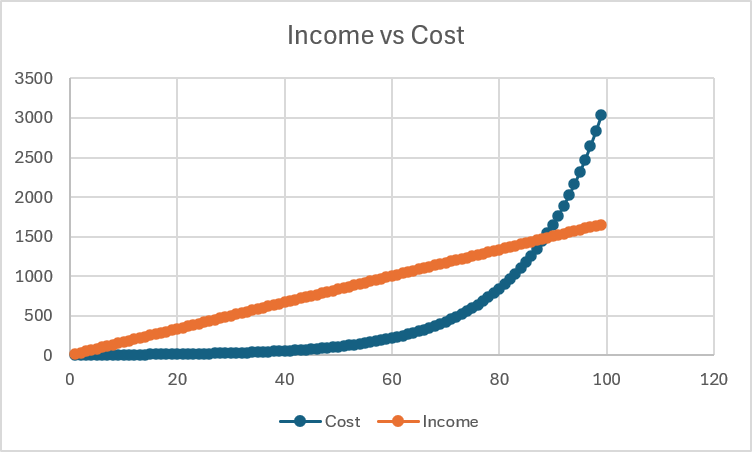
\includegraphics[width=\linewidth]{Figures/IncomeVsCost.png}
  \caption{Polynomial Income vs Exponential Cost}
  \label{fig:income_vs_cost}
\end{figure}
\begin{figure}
  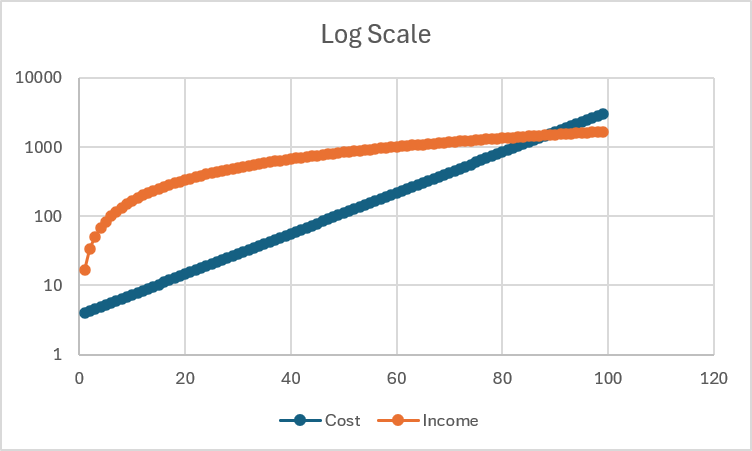
\includegraphics[width=\linewidth]{Figures/LogScale.png}
  \caption{Income vs Cost with y-axes log scaled}
  \label{fig:log_scale}
\end{figure}
\begin{figure}
  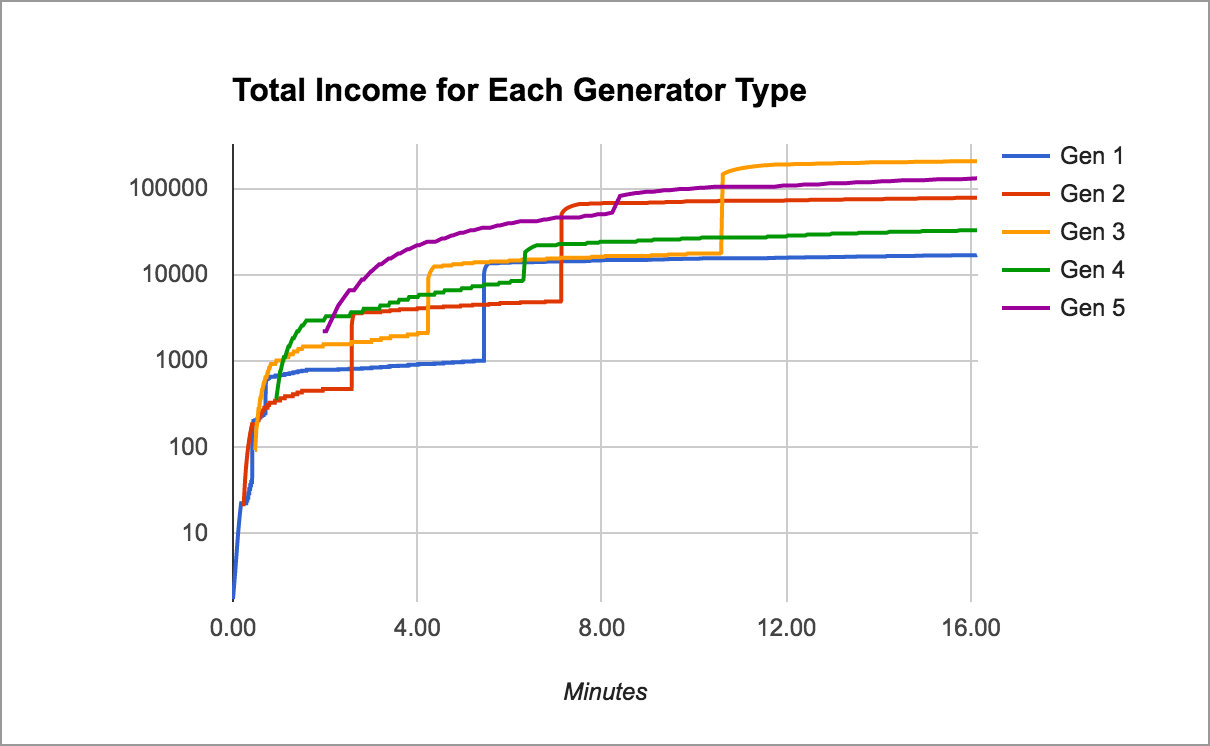
\includegraphics[width=\linewidth]{Figures/InterestingProgression.png}
  \caption{An interesting resource progression}
  \label{fig:interesting_progression}
\end{figure}


%-------------------------------------------------------------------------------
\bibliographystyle{plain}
\bibliography{refs}

%%%%%%%%%%%%%%%%%%%%%%%%%%%%%%%%%%%%%%%%%%%%%%%%%%%%%%%%%%%%%%%%%%%%%%%%%%%%%%%%
\end{document}
%%%%%%%%%%%%%%%%%%%%%%%%%%%%%%%%%%%%%%%%%%%%%%%%%%%%%%%%%%%%%%%%%%%%%%%%%%%%%%%%

%%  LocalWords:  endnotes includegraphics fread ptr nobj noindent
%%  LocalWords:  pdflatex acks
